\documentclass[14pt]{extarticle}
% \documentclass[14pt]{article}

% \usepackage[style=authoryear,maxbibnames=9,maxcitenames=2,uniquelist=false,backend=biber,doi=false,url=false]{biblatex}
% \addbibresource{$BIB} % bibtex location
% \renewcommand*{\nameyeardelim}{\addcomma\space} % have comma in parencite
\usepackage{natbib}

\usepackage{xcolor}
\usepackage{amsmath}
\newcommand{\tuple}[1]{ \langle #1 \rangle }
%\usepackage{automata}
\usepackage{times}
\usepackage{ltablex}
\usepackage{tasks}

%%%%%% Template
\usepackage{hyperref}
\hypersetup{colorlinks=true,allcolors=blue}

\usepackage{vmargin}
\setpapersize{USletter}
\setmarginsrb{1.0in}{1.0in}{1.0in}{0.6in}{0pt}{0pt}{0pt}{0.4in}

% HOW TO USE THE ABOVE:
%\setmarginsrb{leftmargin}{topmargin}{rightmargin}{bottommargin}{headheight}{headsep}{footheight}{footskip}
%\raggedbottom
% paragraphs indent & skip:
\parindent  0.3cm
\parskip    -0.01cm

\usepackage{tikz}
\usetikzlibrary{backgrounds}

% hyphenation:
% \hyphenpenalty=10000 % no hyphen
% \exhyphenpenalty=10000 % no hyphen
\sloppy

% notes-style paragraph spacing and indentation:
\usepackage{parskip}
\setlength{\parindent}{0cm}

% let derivations break across pages
\allowdisplaybreaks

\newcommand{\orange}[1]{\textcolor{orange}{#1}}
\newcommand{\blue}[1]{\textcolor{blue}{#1}}
\newcommand{\red}[1]{\textcolor{red}{#1}}
\newcommand{\freq}[1]{{\bf \sf F}(#1)}
\newcommand{\datafreq}[2]{{{\bf \sf F}_{#1}(#2)}}

\def\qqquad{\quad\qquad}
\def\qqqquad{\qquad\qquad}

%%%%%%%%%%%%%%%%%%%%%%%%%%%%%%%%%%%%%%%%%%%%%%%%%%%%%%%%%%%%%%%%%%%%%%%%%%%%%%%%
%%%%%%%%%%%%%%%%%%%%%%%%%%%%%%%%%%%%%%%%%%%%%%%%%%%%%%%%%%%%%%%%%%%%%%%%%%%%%%%%

% fill-in-blank question style, found in https://tex.stackexchange.com/a/505089

\usepackage{ifthen}
\usepackage{tocloft}
\usepackage{exercise}
% \usepackage{xcolor}

% Set the Show Answers Boolean
\newboolean{showAns}
\setboolean{showAns}{false}
\newcommand{\showAns}{\setboolean{showAns}{true}}

% The length of the Answer line
\newlength{\answerlength}
\newcommand{\anslen}[1]{\settowidth{\answerlength}{#1}}

% ans command that indicates space for an answer or shows the answer in red
\newcommand{\ans}[1]{\settowidth{\answerlength}{\hspace{2ex}#1\hspace{2ex}}%
    \ifthenelse{\boolean{showAns}}%
        {\textcolor{red}{\underline{\hspace{2ex}#1\hspace{2ex}}}}%
        {\underline{\hspace{\answerlength}}}}%

\newcommand{\details}[1]{\settowidth{\answerlength}{#1}%
    \ifthenelse{\boolean{showAns}}%
        {\\ \textcolor{blue}{#1}}%
        {}}%

% Formatting how multiple choices Questions are formated.
\settasks{label=(\Alph*), label-width=30pt}


% Some commands for the Exercise Question package
\renewcommand{\QuestionNB}{\Large\protect\textcircled{\small\bfseries\arabic{Question}}\ }
\renewcommand{\ExerciseHeader}{} %no header
\renewcommand{\QuestionBefore}{3ex} %Space above each Q
\setlength{\QuestionIndent}{8pt} % Indent after Q number


% To create the list of answers with tocloft...
\newcommand{\listanswername}{Answers}
\newlistof[Question]{answer}{Answers}{\listanswername}

% Creates a TOC for Answers
\newcounter{prevQ}
\newcommand{\answer}[1]{\refstepcounter{answer}%
\ans{#1}%
\ifnum\theQuestion=\theprevQ%
        \addcontentsline{Answers}{answer}{\protect\numberline{}#1}% don't include the Q number
        \else%
        \addcontentsline{Answers}{answer}{\protect\numberline{\theQuestion}#1}%
        \setcounter{prevQ}{\value{Question}}%
        \fi%
        }%

% \hyphenpenalty=10000 % no hyphen
% \exhyphenpenalty=10000 % no hyphen
\sloppy              % hyphen

\newcommand{\HRule}{\rule{\linewidth}{0.5mm}}
\newcommand{\Hrule}{\rule{\linewidth}{0.3mm}}

%tocloft formatting listofanswers
\renewcommand{\cftAnswerstitlefont}{\bfseries\large}
\renewcommand{\cftanswerdotsep}{\cftnodots}
\cftpagenumbersoff{answer}
\addtolength{\cftanswernumwidth}{10pt}

\makeatletter% since there's an at-sign (@) in the command name
\renewcommand{\@maketitle}{%
  \parindent=0pt% don't indent paragraphs in the title block
  \centering
  {\Large \bfseries\textsc{\@title}} \\
  \vspace{5pt}
  {\large \textit{\@author}} \\
  \HRule \\
  \vspace{1em}
}
\makeatother% resets the meaning of the at-sign (@)


\title{ECON 2002.01 Midterm Exam }
\author{Hui-Jun Chen}


%%%%%%%%%%%%%%%%%%%%%%%%%%%%%%%%%%%%%%%%%%%%%%%%%%%%%%%%%%%%%%%%%%%%%%%%%%%%%%%%
%%%%%%%%%%%%%%%%%%%%%%%%%%%%%%%%%%%%%%%%%%%%%%%%%%%%%%%%%%%%%%%%%%%%%%%%%%%%%%%%
\begin{document}

\maketitle

% \showAns
% \listofanswer


% \includegraphics[width=\textwidth]{../QuestionBankImage/}

\begin{Exercise}

\Question Which of the following statements is correct regarding disposable income?
\answer{C}

\begin{tasks}(1)
    \task Disposable income is the amount of income that is disposed (given away).
        \details{Disposable income is total income minus transfers to others such as taxes.}
    \task Disposable income is total income, calculated as the sum of an individual's wages, profit, rent, interest, and transfer payments from the government.
        \details{Disposable income is total income minus transfers to others such as taxes.}
    \task Disposable income is the maximum amount of expenditure (e.g. food, housing, clothing, and other goods and services) possible without having to borrow or sell possessions.
        \details{Disposable income is total income minus transfers to others such as taxes, which is the maximum amount of possible expenditure without borrowing or selling.}
    \task Disposable income is the exact measure of one’s wellbeing.
        \details{Disposable income is an insufficient measure of wellbeing, as many aspects of our well-being are not related to what we can buy.}
\end{tasks}

\Question Which of the following does not lead to higher GDP?
\answer{A}

\begin{tasks}(1)
    \task Wealth transfers from the rich to the poor, which lead to higher income equality.
        \details{Equality matters for people’s wellbeing. However, it is not included in a nation’s GDP.}
    \task Higher government expenditure on education.
        \details{GDP includes the goods and services produced by the government, such as education, national defence, and law enforcement.}
    \task Rebuilding and reopening an abandoned shopping mall, which is immediately occupied by new businesses.
        \details{The activities of firms are counted as part of GDP.}
    \task Building a new manufacturing factory, which requires the clearing of forests.
        \details{Environmental damage is not reflected in GDP, but the building of a factory is.}
\end{tasks}

\Question Which of the following statements is correct?
\answer{C}

\begin{tasks}(1)
    \task A model is an exact representation of what goes on in the economy.
        \details{A model is a simplified representation that helps to understand what happens in the economy.}
    \task A model is an economic relationship that is only represented by mathematics.
        \details{While mathematics is part of the language of economics, much of the knowledge of economics cannot be expressed in mathematics but instead requires either verbal or graphical representations.}
    \task Equilibrium is a self-perpetuating situation that does not change, unless a force for change is introduced from the outside and alters the basic data describing the situation.
        \details{This is the definition of equilibrium.}
    \task Equilibrium in GDP growth rate is when the growth rate is zero.
        \details{A non-zero rate of change can be an equilibrium if it does not change in the absence of some external force.}
\end{tasks}

\Question In the following diagram you are given two technologies, A and B, which can produce 100 metres of cloth. Technology A uses 1 worker and 4 tonnes of coal, while technology B uses 4 workers and 2 tonnes of coal. The diagram also depicts three examples of isocosts, NM, GF and JH. The wage cost and the price of coal are denoted by wand p, respectively. In case 1, the wage cost and the price of coal are (w, p) = (20, 10), while in case 2, (w, p) = (10, 20). Which of the following statements is correct?
\answer{B}

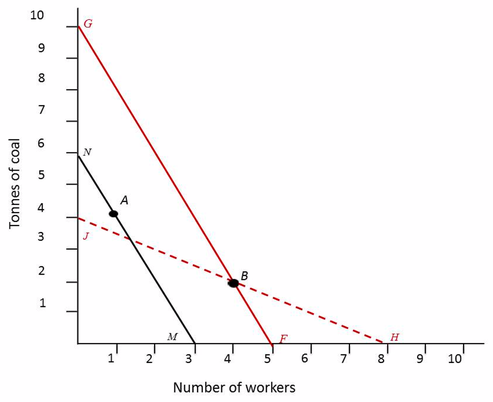
\includegraphics[width=\textwidth]{../QuestionBankImage/OUP-U2-Q11-01.png}

\begin{tasks}(1)
    \task Technology B would be chosen in both cases 1 and 2.
        \details{Isocosts NM and GF correspond to case 1 while isocost JH corresponds to case 2. In case 1, the isocost NM going through A is lower than the isocost GF going through B (due to lower total cost). This implies that A would be chosen instead of B in case 1.}
    \task Technology A would be chosen in case 1 while technology B would be chosen in case 2.
        \details{Isocosts NM and GF correspond to case 1 while isocost JH corresponds to case 2. In case 1 the lower isocost goes through A, implying that A would be chosen. Similarly in case 2, isocost JH would be lower than the corresponding isocost that would go through A, and therefore B would be chosen.}
    \task Technology B would be chosen in case 1 while technology A would be chosen in case 2.
        \details{Isocosts NM and GF correspond to case 1 while isocost JH corresponds to case 2. In case 1 technology A would be chosen, while in case 2 technology B would be chosen.}
    \task Technology B would be cheaper under case 1 than under case 2.
        \details{Under case 1 the cost of technology B is c = (\$20 × 4) + (\$10 × 2) = \$100. Under case 2 the cost is c = (\$10 × 4) + (\$20 × 2) = \$80. Therefore technology B is cheaper under case 2.}
\end{tasks}

\Question Which of the following statements regarding the Malthusian model are correct when there is a positive one-off technological shock (such as an improved seed)?
\answer{C}

\begin{tasks}(1)
    \task There is an immediate and permanent rise in the average product of labour.
        \details{A key assumption of the Malthusian model is the diminishing average product of labour as population rises.}
    \task The population initially rises but then falls to the pre-technological shock level.
        \details{The population settles at a higher level as a result of the positive technological shock.}
    \task Income initially rises but then falls to the subsistence level in equilibrium.
        \details{Subsistence level is the level at which there is no population growth. This is the equilibrium.}
    \task Malthus’ Law states that an increase in productivity will result in both increased population and wages in the long run.
        \details{Malthus’ Law states that an increase in productivity will result in a larger population but not increased wages in the long run.}
\end{tasks}

\Question Which of the following is an economic rent?

\answer{C}
\begin{tasks}(1)
    \task The amount you pay your landlord for the use of an apartment.
        \details{This is the rent as used in everyday language. Economic rent is something you would like to get and not something you have to pay.}
    \task The amount you pay to hire a car for a weekend.
        \details{An economic rent is what you earn above the next best alternative, which in this case may be the additional earnings compared to subletting the land to someone else at the same rate.}
    \task The extra profit that a successful innovator makes on bringing a new product to the market before its competitors.
        \details{This particular form of economic rent is called an innovation rent, where profits are made in excess of those offered by the next best alternative due to the adoption of new technology.}
    \task The extra profit that a firm makes when it doubles in size and there are no changes to costs or the price for each unit of its output.
        \details{This would be the normal profit you can earn in return for hard work. An economic rent is what you earn over and above the next best option, for example working really hard in another job.}
\end{tasks}

\Question You currently work for 40 hours a week at wage rate of £12 an hour. Your free hours are defined as the number of hours not in work, which in this case is 24 hours × 7 days – 40 hours = 128 hours per week. Suppose that you are happy to keep your total weekly income constant. Then:
\answer{B}
\begin{tasks}(1)
    \task If your wage rate increases to £16 an hour, then your free time will increase by 6\%.
        \details{The current total weekly income is £12 × 40 hours = £480. At the wage rate of £16, you will only need to work for 480 /16 = 30 hours a week. This will increase your free time to 138 hours, which is an increase of (138 – 128) / 128 = 7.8\%.}
    \task To have 12.5\% more free time, your wage rate needs to increase by £8.
        \details{The current total weekly income is £12 × 40 hours = £480. 12.5\% extra free time means 128 hours × 1.125 = 144 hours of free time, or 24 hours of work. To keep your weekly income constant, your wage rate needs to increase to £480 / 24 = £20 an hour, which is an increase of £8.}
    \task Doubling the wage rate would decrease your working hours by a third.
        \details{The current total weekly income is £12 × 40 hours = £480. If the wage rate doubles to £24, your working hours fall to 480 /24 = 20 hours a week, i.e. it halves.}
    \task A wage cut of 25\% leaves you with only 100 hours of free time.
        \details{The current total weekly income is £12 × 40 hours = £480. A wage cut of 25\% means your new hourly wage is £12 × (1 – 0.25) = £9. To keep the weekly income constant you will have to work 480 ÷ 9 = 53 hours and 20 minutes, which leaves you with 114 hours and 40 minutes of free time.}
\end{tasks}

\Question  The figure shows the indifference curves of a student for the two ‘goods’, free time and final grade. Based on this information, which of the following statements is correct?
\answer{A}
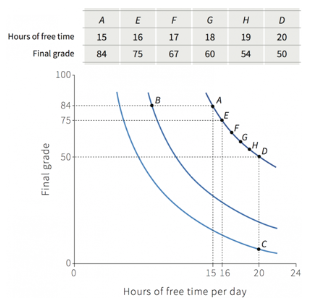
\includegraphics[width=\textwidth]{../QuestionBankImage/OUP-U3-Q9-01.png}
\begin{tasks}(1)
    \task At A, the student is willing to give up 34 grade points for five extra hours of free time.
        \details{This is true, as points A and D are on the same indifference curve.}
    \task A is the student’s most preferred choice as she would be attaining the highest grade.
        \details{The student is indifferent between A and all the other points on the same indifference curve i.e. E, F, G, H, and D.}
    \task The student strictly prefers a grade of 54 with 19 hours of free time to a grade of 67 with 18 hours of free time.
        \details{A grade of 54 with 19 hours of free time is point H. The student is indifferent between this point and point F, where she gets a grade of 67 with 17 hours of free time. She would therefore strictly prefer a grade of 67 with 18 hours of free time to H.}
    \task If at B the number of free hours is 10, then the student is 50\% happier at A than at B.
        \details{Higher indifference curves imply higher levels of utility, but the specific level of utility depends on the student’s relative preferences for both goods. It is not necessarily true that 50\% additional free time would make the student 50\% happier.}
\end{tasks}

\Question You have two choices for how you are going to spend Saturday evening. You can go to the pub with your friends, which will cost you £30 for the evening. The pleasure you anticipate from this experience is worth £50 to you. Or you can go to the theatre. The ticket will cost you £50, but you value the experience at £60. Based on this information, which of the following statements is correct?
\answer{C}
\begin{tasks}(1)
    \task The opportunity cost of an evening at the theatre is £10.
        \details{The opportunity cost of an evening at the theatre is the economic rent of the alternative, which is going to the pub. This is £50 – £30 = £20.}
    \task The economic cost of going to the theatre is £60.
        \details{The economic cost of going to the theatre is the sum of the accounting cost and the opportunity cost, which in this case is £50 + £20 = £70.}
    \task The economic rent of going to the theatre is -£10.
        \details{The economic rent is the difference between the value of the experience and its economic cost, which here is £60 – £70 = -£10.}
    \task Based on economic rent alone, you would choose to go to the theatre.
        \details{The economic rent for the theatre is negative at -£10, whereas the economic rent for the pub is positive at £10. Therefore you would choose to go to the pub instead of the theatre.}
\end{tasks}

\Question  Consider a worker whose choice is between hours of free time and consumption. His company has now cut his wage rate. Which of the following statements is correct?
\answer{C}
\begin{tasks}(1)
    \task As a result of the substitution effect, the worker would reduce his free time.
        \details{A wage cut implies a fall in the opportunity cost of free time. Therefore the worker would increase his free time as a result of the substitution effect.}
    \task The income effect means that the worker would increase his free time.
        \details{The worker’s total income will fall as a result of the wage cut. This implies a negative income effect.}
    \task The worker may or may not reduce his free time as a result of the wage cut.
        \details{The worker will increase his free time if the positive substitution effect dominates the negative income effect. On the other hand, if the income effect dominates the substitution effect, then he will reduce his free time.}
    \task The income effect will always dominate the substitution effect of the wage cut.
        \details{Whether the income effect dominates the substitution effect or not depends on the shape of the worker’s indifference curves.}
\end{tasks}

\Question Figure 3.6 shows Alexei’s indifference curves for free time and final grade. Which of the following is true?
\answer{B}
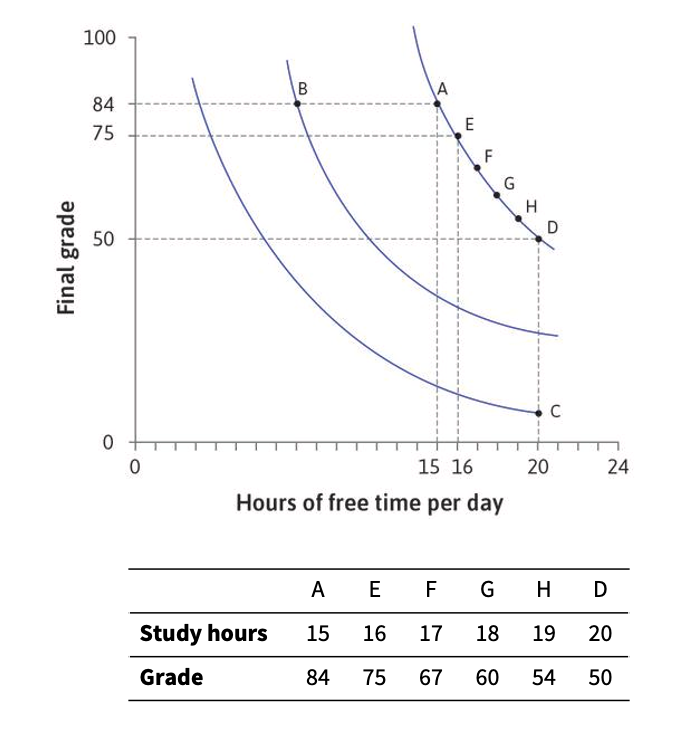
\includegraphics[width=\textwidth]{../QuestionBankImage/ECO-U3-Q4-01.png}
\begin{tasks}(1)
    \task Alexei prefers C to B because at C he has more free time.
        \details{The indifference curve through C is lower than that through B. Hence Alexei prefers B to C.}
    \task Alexei is indifferent between the grade of 84 with 15 hours of free time, and the grade of 50 with 20 hours of free time.
        \details{A, where Alexei has the grade of 84 and 15 hours of free time, and D, where Alexei has the grade of 50 with 20 hours of free time, are on the same indifference curve.}
    \task Alexei prefers D to C, because at D he has the same grade and more free time.
        \details{At D Alexei has the same amount of free time but a higher grade.}
    \task At G, Alexei is willing to give up 2 hours of free time for 10 extra grade points.
        \details{The opposite trade-off is true: going from G to D, Alexei is willing to give up 10 grade points for 2 extra hours of free time. Going from G to E, he is willing to give up 2 hours of free time for 15 extra grade points.}
\end{tasks}

\Question The following diagram is the feasible set of a student, showing the combinations of her final grade and the hours of free time per day. Based on this information, we can say that:
\answer{D}
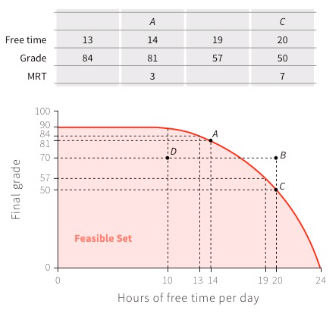
\includegraphics[width=\textwidth]{../QuestionBankImage/OUP-U3-Q15-01.png}
\begin{tasks}(1)
    \task Whether the student would choose A or B depends on her preferences.
        \details{B is outside the feasible set and therefore can never be chosen.}
    \task At A, the student can attain grade of 81 for 14 hours of study.
        \details{At A, the student is able to attain a grade of 81 and have 14 hours of free time, so she studies for 10 hours.}
    \task C would never be chosen over A.
        \details{The student can choose C over A if her indifference curves are steep enough.}
    \task The marginal rate of transformation increases with higher number of free hours.
        \details{For a higher number of free hours, sacrificing one hour of free time gives a larger increase in grade points.}
\end{tasks}

\Question
Which of the following statements regarding employment contracts are correct?
\answer{C}
\begin{tasks}(1)
    \task
The firm is required to state exactly what it needs the employee to do in an employment contract.
        \details{
Due to unforeseen future events, the firm cannot possibly know exactly what it will need the employee to do at the time the contract is signed.
        }
    \task
	The firm needs to specify exactly how much effort employees are expected to put into their job.
        \details{
It is impractical or too costly for the firm to observe exactly how much effort each employee puts into their job.
        }
    \task
Employees’ effort levels cannot be the basis of an enforceable contract.
        \details{
This is true – for example, a restaurant owner cannot take an employee to a court to decide whether he can withhold wages because the waiter had not smiled often enough.
        }
    \task
Employment contracts are incomplete as they can only specify things that both the employees and the business owner care about.
        \details{
Employment contracts are incomplete as they cannot specify things that both the employees and the business owner care about: how hard and well the employee will work, and for how long the worker will stay.
        }
\end{tasks}

\Question
Thomas earns £12 per hour in his current job and works 36 hours a week. He loves his job and puts in his maximum effort with no disutility. In fact, Thomas earns extra utility worth £3 per hour from camaraderie, status, and enjoyment of the job. If he loses this job Thomas has two choices. Either he is able to be self-employed, which earns him £7 an hour for 36 hours a week of work but also gives him disutility equivalent to £2 per hour, or he can be unemployed and receive an unemployment benefit of £150 per week. Thomas is expected to be able to find another job similar to his current one in 24 weeks. Then:
\answer{D}
\begin{tasks}(1)
    \task
Thomas’s next best option is to be unemployed.
        \details{
By being self-employed he will receive a benefit of (7 – 2) × 36 = £180 per week. This is higher than the unemployment benefit of £150 per week.
        }
    \task
The employment rent per hour is £8.
        \details{
The employment rent is (12 + 3) – (7 – 2) = £10 per hour.
        }
    \task
Thomas’s employment rent is £9,360.
        \details{
The employment rent is (12 + 3) – (7 – 2) = £10 per hour for 36 hours a week over the expected unemployment duration of 24 weeks i.e. 10 × 36 × 24 = £8,640.
        }
    \task
If Thomas chooses the self-employment option then his loss of employment rent is £8,640.
        \details{
		The loss of employment rent is the rent between the current job and self-employment. This is (12 + 3) – (7 – 2) = £10 per hour for 36 hours a week over the expected unemployment duration of 24 weeks i.e. 10 × 36 × 24 = £8,640.
        }
\end{tasks}

\Question
Consider isocost lines drawn on a graph with hourly wage on the horizontal axis and effort per hour on the vertical axis. Which of the following statements is correct?
\answer{D}
\begin{tasks}(1)
    \task
Isocost lines intersect the horizontal axis at the reservation wage.
        \details{
Isocost lines go through the origin (zero wage, zero cost).
        }
    \task
The slope of the isocost line is the employer’s marginal rate of transformation of higher wages into worker effort.
        \details{
The slope of the isocost lines is the employer’s marginal rate of substitution, which is the rate at which the employer is willing to increase wages to get higher effort.
        }
    \task
Steeper isocost lines represent higher cost per unit of effort.
        \details{
The slope of the isocost lines represents the units of effort per dollar of wage cost. Steeper isocosts therefore mean more units of effort per dollar of wage cost, or equivalently, a lower cost per unit of effort.
        }
    \task
For an isocost lines with a slope of 0.07, the cost of unit of effort is \$14.3.
        \details{
The slope of the isocost lines represents the units of effort per dollar of wage cost, which is the inverse of the cost per unit of effort. The latter is therefore 1/0.07 = \$14.3.
        }
\end{tasks}

\Question
If unemployment benefits increase:
\answer{C}
\begin{tasks}(1)
    \task
A worker’s effort increases because the employment rent increases.
        \details{
The lost income relative to being employed falls, so the employment rent decreases and a worker’s effort decreases.
        }
    \task
Effort decreases because the disutility of effort decreases.
        \details{
Effort decreases because the employment rent decreases.
        }
    \task
The employment rent will fall unless the firm raises the wage.
        \details{The lost income relative to being employed falls, so the employment rent decreases, unless the firm increases the wage.}
    \task
The employment rent will increase unless the firm raises the wage.
        \details{The lost income relative to being employed falls, so the employment rent decreases, unless the firm increases the wage.}
\end{tasks}

\Question
    Which of the following statements best describes the game played by the employer and the employee in the labour discipline model?
\answer{C}
\begin{tasks}(1)
    \task
The game is a simultaneous game in which the employer chooses the wage level and the employee chooses the effort level simultaneously.
        \details{
The game is a sequential game where the employer, knowing the employee’s possible decisions, selects the wage level first. The employee then selects his effort level given the offered wage level.
        }
    \task
The game is a one-off game in which the wage and effort levels are determined once and for all.
        \details{
The game is a repeated game where wages and effort levels decisions are made in each period.
        }
    \task
	The worker selects the effort level that balances his desire to keep his job with his desire to not exhaust himself on the job.
        \details{
    In the labour discipline model, putting in effort is costly for the worker, but he earns an employment rent from keeping his job. The amount of effort chosen depends on the relative size of these effects.
        }
    \task
The employer will attempt to maximise the firm’s profits by offering a wage equal to the worker’s reservation wage.
        \details{At his/her reservation wage, the worker will have no incentive to exert any effort. Therefore this will not be the firm’s optimal strategy.}
\end{tasks}


\Question
Maria earns \$12 per hour in her current job and works 35 hours a week. Her disutility of effort is equivalent to a cost of \$2 per hour of work. If she loses her job, she will receive unemployment benefit equivalent to \$6 per hour. Additionally, being unemployed has psychological and social costs equivalent to \$1 per hour. Then:
\answer{D}
\begin{tasks}(1)
    \task
The employment rent per hour is \$3.
        \details{
Employment rent per hour = wage – unemployment benefit – disutility of effort + disutility of unemployment = 12 – 6 – 2 + 1 = \$5. This is the net hourly benefit of being employed compared with unemployment.
        }
    \task
Maria’s reservation wage is \$6 per hour.
        \details{
Maria’s reservation wage = unemployment benefit – disutility of unemployment = 6 – 1 = \$5. This is the wage at which Maria is just willing to forgo her unemployment benefits for a job (but it is not enough to make her put in effort!).
        }
    \task
Maria’s employment rent if she can get another job with the same wage rate after 44 weeks of being unemployed is \$6,160.
        \details{
Maria’s employment rent = \$5 (employment rent per hour) × 35 hours per week × 44 weeks = \$7,700.
        }
    \task
Maria’s employment rent if she can only get a job at a lower wage rate after 44 weeks of being unemployed is more than \$7,700.
        \details{
If she could get a job at the same wage after 44 weeks, Maria’s employment rent = \$5 (employment rent per hour) × 35 hours per week × 44 weeks = \$7,700. If the new job would have a lower wage, her employment rent would be higher than \$7,700.
        }
\end{tasks}

\Question
Which of the following statements regarding the marginal rate of substitution (MRS) and the marginal rate of transformation (MRT) of a profit-maximising firm is correct?
\answer{A}
\begin{tasks}(1)
    \task
	The MRS is how much in price you are willing to give up for an incremental increase in the quantity, holding profits constant.
        \details{This is the definition of the MRS. It is the slope of the isoprofit curves.}
    \task The MRT is how much in price the consumers are willing to give up for an incremental increase in the quantity consumed, keeping their utility constant.
        \details{The MRT is how much the firms have to drop the price for an incremental increase in demand. It is the slope of the demand curve.}
    \task If MRT $>$ MRS then firms can increase their profit by increasing output.
        \details{When MRT $>$ MRS, the slope of the demand curve is steeper than the slope of the isoprofit curve that intersects the demand curve. This means that for a unit decrease in output, firms are able to increase the price more than the amount required to keep their profit constant. Therefore to increase profit, they should decrease output.}
    \task The MRT is the slope of the isoprofit curves.
        \details{The MRT is the slope of the demand curve.}
\end{tasks}

\Question
Which of the following statements regarding average cost and marginal cost of a firm is correct?
\answer{D}
\begin{tasks}(1)
    \task
	Average cost is the slope of the total cost curve.
        \details{Average cost is the slope of the ray from the origin to a point on the total cost curve.}
    \task
	Marginal cost is the slope of the average cost curve.
        \details{Marginal cost is the slope of the total cost curve.}
    \task
	Marginal cost is always higher than average cost.
        \details{When average cost decreases with output, marginal cost is lower than the average cost.}
    \task
	When marginal cost equals average cost, the slope of the average cost curve is zero.
        \details{When marginal cost equals average cost, the cost of producing one extra unit of output is the same as the average of the costs of producing all existing outputs. This keeps the average the same, so the average cost curve is horizontal at this point.}
\end{tasks}

\Question
The figure depicts the demand curve of a firm producing cars, together with its marginal cost, average cost, and isoprofit curves. Based on the figure, which of the following statements is correct?
\answer{C}
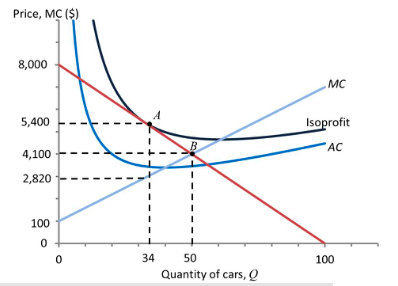
\includegraphics[width=\textwidth]{../QuestionBankImage/OUP-U7-Q22-01.png}

\begin{tasks}(1)
    \task
The consumer surplus in the profit-maximising outcome is \$105,300.
        \details{The profit-maximising outcome is A. The consumer surplus is ½ × (8000 – 5400) × 34 = \$44,200. \$105,300 is the consumer surplus at the Pareto efficient outcome B.}
    \task
	The producer surplus in the Pareto efficient outcome is \$133,960.
        \details{The Pareto-efficient outcome is B. The producer surplus is ½ × (4000 – 100) × 50 = \$100,000. \$133,960 is the producer surplus at the profit-maximising outcome A.}
    \task
	The deadweight loss in the profit-maximising outcome is \$20,640.
        \details{The profit-maximising outcome is A. The deadweight loss is ½ × (5400 – 2820) × (50 – 34) = \$20,640.}
    \task
    	The firm’s profit in the Pareto efficient outcome is \$100,000.
        \details{The Pareto-efficient outcome is B. \$100,000 is the producer surplus at this point. The firm’s profit is producer surplus minus its fixed costs, so is less than \$100,000}
\end{tasks}

\Question
The following figure depicts a firm’s profit-maximisingchoice at point E, given the market demand curve and the firm’s marginal cost curve. You are given that the firm’s marginal costs are \$400, \$2,960 and \$4,200 at output levels Q = 0, Q* = 32 (point E) and $Q_0= 48$ (point F), respectively. Based on this information, which of the following statements is correct?
\answer{C}
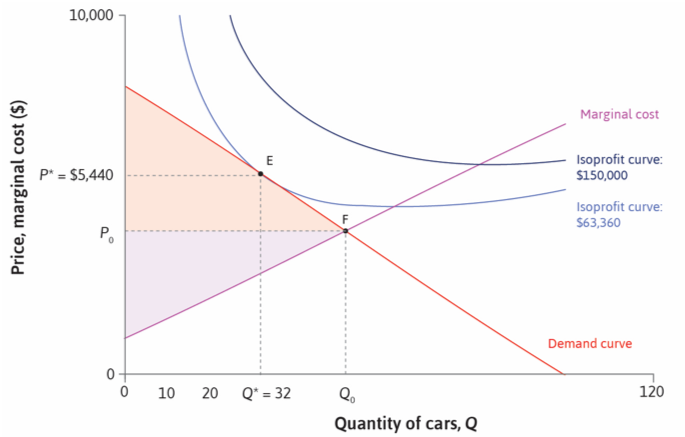
\includegraphics[width=\textwidth]{../QuestionBankImage/TEA-U7-Q5-01.png}

\begin{tasks}(1)
    \task
	The consumer surplus at E is \$41,000.
        \details{The consumer surplus at E is (1/2) x (7920 – 5440) x 32 = \$39,680.}
    \task
	The producer surplus at E is \$126,720.
        \details{The producer surplus at E is (1/2) x (2480 + 5040) x 32 = \$120,320.}
    \task
	The deadweight loss at E is \$19,840.
        \details{The deadweight loss at E is (5440 – 2960) x (48 – 32) x (1/2) = \$19,840.}
    \task
	The gains from trade at E are \$120,320.
        \details{The gains from trade at E are the sum of consumer surplus and producer surplus: CS + PS = 39,680 + 120,320 = \$160,000.	}
\end{tasks}

\Question
 Demand faced by a monopolist is Q = 20 – 0.5P. Her marginal cost is 10. Based on this information we can say that:
\answer{C}
\begin{tasks}(1)
    \task
	The optimal production of the monopolist is Q = 15.
        \details{The monopolist will produce until MR = MC. From the demand function, we find that P = 40 - 2Q. Therefore, revenue R is $R = Q \times  P = 40Q - 2Q^2$. Marginal revenue MR is: $dR/dQ = MR = 40 - 4Q$. Because MR = MC, then 40 - 4Q = 10 which implies that Q* = 7.5. So the monopolist will produce 7.5 units.}
    \task
	The price charged by the monopolist is equal to her marginal cost.
        \details{This would be true in case of perfect competition. In this case, the price is obtained through the inverse demand function: P* = 40 - 2Q* = 40 - 2 x 7.5 = 25.}
    \task
	The deadweight loss associated with the monopolist’s choice of price is less than the product of the difference between her price and marginal cost, multiplied by her optimal quantity.
        \details{The deadweight loss (DWL) associated with the monopolist's choice is DWL = (1/2) x ((25 - 10) x (15 - 7.5)) = 56.25. The product of the difference between her price and marginal cost multiplied by her optimal quantity is given by (25 - 10) x 7.5 = 112.5.}
    \task
	The price charged by the monopolist is lower to her marginal cost.
        \details{If the price is lower than marginal cost then she is incur a loss for every unit sold. So this is wrong.}
\end{tasks}

\Question
 Consider a firm with fixed costs of production. Which of the following statements about its average cost (AC) and marginal cost (MC) is correct?
\answer{A}
\begin{tasks}(1)
    \task
When $AC = MC$, the AC curve has a zero slope.
        \details{When AC = MC, the cost of an additional unit equals the average cost of all existing units. Therefore, the new AC will be the same and the slope is zero.}
    \task
	When $AC > MC$, the MC curve is downward-sloping.
        \details{The MC curve can be upward-sloping, horizontal, or downward-sloping, irrespective of the relative size of AC and MC.}
    \task
	When $AC < MC$, the AC curve is downward-sloping.
        \details{When $AC < MC$, the cost of an additional unit is greater than the average cost of the existing outputs. So the new AC will be larger. The AC curve is upward-sloping.}
    \task
	The MC curve cannot be horizontal.
        \details{If MC is constant, then the MC curve is horizontal.}
\end{tasks}

\Question
This figure shows the marginal cost and marginal revenue curves for Beautiful Cars. Which of the following statements is correct, based on the information shown?
\answer{D}

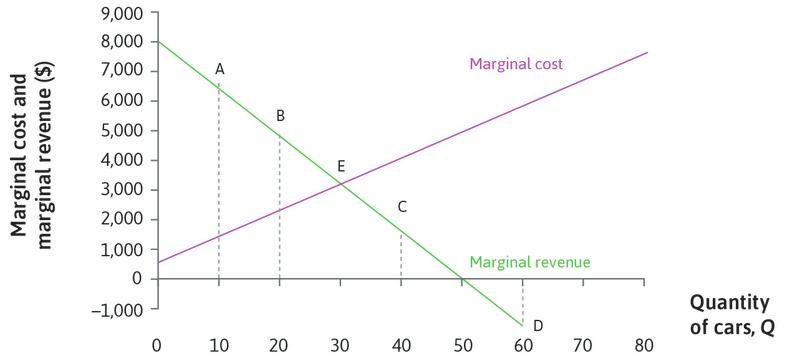
\includegraphics[width=\textwidth]{../QuestionBankImage/ECO-U7-Q12-01.jpg}
\begin{tasks}(1)
    \task
When Q = 40, the marginal cost is greater than the marginal revenue so the firm’s profit must be negative.
        \details{When Q = 40 the marginal cost is greater than the marginal revenue so the marginal profit is negative. This doesn’t mean that profit is negative.}
    \task
	Revenue is greater when Q = 10 than if Q = 20.
        \details{The marginal revenue is greater at Q = 10 than Q = 20. But because the marginal revenue is positive as output increases from 10 to 20, revenue is increasing: it is higher at Q = 20.}
    \task
	The firm would not choose to produce at point E because marginal profit is zero.
        \details{Marginal profit is zero at E. But this is the profit-maximizing point, so the firm will choose it.}
    \task
    	Profit is greater when Q = 20 than when Q = 10.
        \details{At all levels of output up to point E, marginal revenue is greater than marginal cost. So profit increases as output increases—it is higher at Q = 20 than Q = 10.	}
\end{tasks}

\Question
The figure shows the wage-setting curve and the real wage w*. Which of the following statements is correct?
    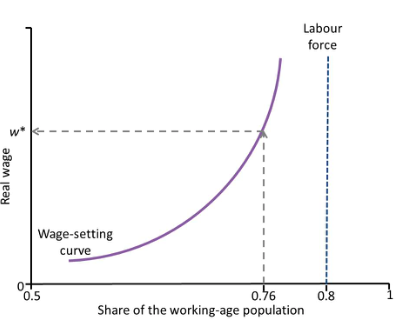
\includegraphics[width=\textwidth]{../QuestionBankImage/OUP-U9-Q3-01.png}
\answer{A}
\begin{tasks}(1)
    \task The unemployment rate is 5\%.
        \details{Unemployment rate = Unemployed / Labour force = (0.8 – 0.76)/0.8 = 5\%.}
    \task The participation rate is 76\%.
        \details{Participation rate = Labour force / Population of working age = 0.8 or 80\%.}
    \task The employment rate is 95\%.
        \details{Employment rate = Employed / Population of working age = 0.76 or 76\%.}
    \task 4\% of the population is unemployed.
        \details{Here we do not know the size of the population. However the population is bigger than the working-age population, and therefore the proportion of the population unemployed is less than 4\%.}
\end{tasks}

\Question
Which of the following statements about the wage-setting curve is correct?
\answer{B}
\begin{tasks}(1)
    \task
The wage-setting curve depicts the workers’ reservation wage for different levels of economy-wide employment.
        \details{The wage-setting curve depicts the real wage necessary to provide workers with incentives to work hard (which is higher than their reservation wage), for different levels of economy-wide employment.}
    \task
At each point (U, w) on the wage-setting curve, the workers are choosing their best response effort level given the real wage (w) and unemployment rate (U).
        \details{This is true. Each point (U, w) on the wage-setting curve is derived as the point of tangency between the workers’ best response function (their best choice of effort per hour for each w, given U) and the employers’ isocost line.}
    \task
A lower unemployment rate shifts the wage-setting curve to the left.
        \details{A lower unemployment rate shifts the workers’ best response function for effort exerted given the wage level to the right. This means that the employers need to offer a higher wage to induce a higher effort level. This is a movement up along the wage-setting curve and not a shift of the entire curve, since employment is endogenous (the horizontal axis variable).}
    \task
An exodus of European workers due to Brexit would, ceteris paribus, result in a downward shift of the UK’s wage-setting curve.
        \details{With the balance of job seekers and vacancies shifting in favour of the remaining workers, their best response function shifts to the right, resulting in the wage-setting curve shifting up.}
\end{tasks}

\Question
Which of the following statements about the price-setting curve is correct?
\answer{C}
\begin{tasks}(1)
    \task
The price-setting curve depicts the firms’ profit-maximising price level for different levels of economy-wide employment.
        \details{The price-setting curve depicts the real wage paid when firms choose their profit-maximising price, for different levels of economy-wide employment.}
    \task
Firms have to pay a higher real wage when the employment rate is higher. Therefore the price-setting curve is upward-sloping.
        \details{The price-setting curve represents the level of the real wage consistent with the firms’ profit-maximising markup over costs. It is independent of the level of employment in the economy, and therefore it is a horizontal line.}
    \task
At points below the price-setting curve, the firms are setting prices too high compared to their profit-maximising level.
        \details{The price-setting curve represents the profit-maximising real wage. At points below the curve the real wage is lower than the level consistent with the firm’s profit-maximising markup, and therefore the markup, and hence the price, is too high.}
    \task
The reduction in competition from Europe due to Brexit would result in the UK’s price-setting curve shifting up.
        \details{Lower competition means a higher markup. With the workers’ APL unaffected this leads to a fall in the real wage. Therefore the price-setting curve shifts down.}
\end{tasks}

\Question
Consider an economy with firms selling differentiated products, where the only input to production is labour. Which of the following statements is correct?
\answer{D}
\begin{tasks}(1)
    \task Firms make no economic rent.
        \details{With differentiated products, firms make profits above normal profits.}
    \task Workers receive no employment rent.
        \details{A positive economic rent is required in order to induce workers to exert effort.}
    \task Firms choose the level of nominal wage that corresponds to the workers’ maximum effort.
        \details{Firms choose the lowest nominal wage they can pay without undermining the workers’ motivation to work. It may not be optimal for firms to choose a high wage even if it increases worker effort, because costs may increase more than revenues (hence profits may fall).}
    \task
	The more inelastic the demand curve faced by the firm, the higher the markup set by the firm.
        \details{Inelastic demand means a steeper demand curve, so the firm has more market power. Therefore it is able to set a higher markup.}
\end{tasks}


\Question
The figure depicts the labour market when there has been a negative aggregate demand shock. Which of the following statements is correct?
\answer{A}
    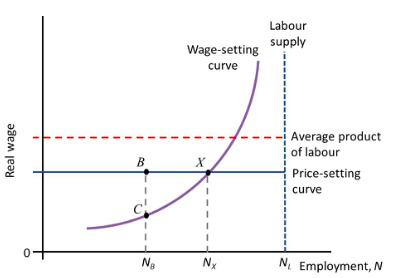
\includegraphics[width=\textwidth]{../QuestionBankImage/OUP-U9-Q17-01.png}
\begin{tasks}(1)
    \task B is not a Nash equilibrium outcome.
        \details{B is above the wage-setting curve. This means that the firms are able to increase profits by reducing their wage offer, without incurring a loss in the effort exerted by the workers. Therefore, given workers' behaviour, firms are not choosing their optimal response at B i.e. B is not a Nash equilibrium.}
    \task C is a Nash equilibrium outcome.
        \details{C is below the price-setting curve. This means that the firms are able to increase profits by restoring their profit-maximising markup away from C. Therefore it is not a Nash equilibrium.}
    \task At C, firms are able to make higher profits by increasing the price.
        \details{At C, the real wage is too low. Therefore the firms would reduce their price to re-attain their profit-maximising markup.}
    \task Moving from B to C eliminates cyclical unemployment.
        \details{Cyclical unemployment is $N_X - N_B$, which is not eliminated by moving from B to C}
\end{tasks}

\Question
Which of the following statements is correct?
\answer{C}
\begin{tasks}(1)
    \task Human capital is the physical capital owned by humans.
        \details{Human capital refers to non-tangible endowments such as knowledge, skills, and abilities, which determine your labour productivity and earnings. Human capital does not refer to physical assets.}
    \task Wealth and income are both stock variables.
        \details{Wealth is a stock variable as it has no time dimension and consists of what an entity owns at a particular point in time. On the other hand, income is a flow variable as it is the amount of money received over some period of time.}
    \task Depreciation is a flow variable.
        \details{Depreciation is the reduction in the value of a stock of wealth over time. Therefore it is a flow variable.}
    \task Net income is before-tax income minus tax.
        \details{Net income is after-tax income minus depreciation.}
\end{tasks}


\Question
The diagram depicts Mary's choice of consumptions in periods 1 and 2. She has no income in period 1 and an income of \$100 in period 2. In scenario 1 the interest rate is 78\%, while in scenario 2 it falls to 10\%. Based on this information, which of the following statements is correct?
    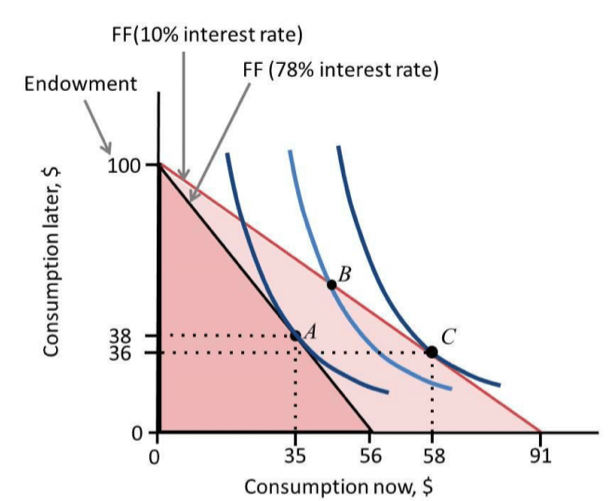
\includegraphics[width=\textwidth]{../QuestionBankImage/OUP-U10-Q8-01.png}

\answer{B}
\begin{tasks}(1)
    \task In scenario 1, Mary is better off choosing B than A.
        \details{B is not a feasible option under scenario 1.}
    \task The substitution and income effects of the interest rate fall work in the opposite directions for consumption in period 2.
        \details{The substitution effect would encourage Mary to consume less in period 2 (cheaper borrowing costs for period 1 consumption), while the income effect would encourage Mary to consume more in period 2.}
    \task The fall in the interest rate always results in a rise in consumption in both periods.
        \details{This is true for period 1 consumption, where substitution and income effects work in the same direction. For period 2 consumption, they work in opposite directions and may results in a fall in consumption if the substitution effect dominates the income effect (as depicted in this case).}
    \task Mary is more impatient at her optimal choice after the interest rate fall.
        \details{The marginal rate of substitution is lower at C than at A. Therefore she is less impatient after the rate fall.}
\end{tasks}


\Question
The diagram depicts Marco’s choice of consumptions in periods 1 and 2. He has \$100 worth of grain in period 1 and no income in period 2. Marco decides to consume \$65 worth of grain in period 1, sell the remaining grain and lend the money at an interest rate of 10\%, which he uses to buy grain for his consumption in period 2 (point A). Which of the following statements regarding his balance sheet is correct?

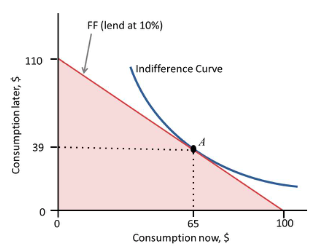
\includegraphics[width=\textwidth]{../QuestionBankImage/OUP-U10-Q15-01.png}

\answer{D}
\begin{tasks}(1)
    \task The asset after lending but before consumption is \$65.
        \details{Even when he has lent the money, the money remains on the balance sheet as an asset. Therefore the asset after lending but before consumption is \$100.}
    \task The asset after consumption in period 1 is \$39.
        \details{The asset after consumption in period 1 is the amount that Marco has saved, which is \$35.}
    \task The net worth before consumption in period 2 is \$0.
        \details{Marco’s assets in period 2 before consumption is \$39. He has no liabilities. Therefore his net worth is \$39.}
    \task Marco’s liabilities remain at 0 at all times.
        \details{In this scenario Marco does not borrow at all at any time. Therefore his liability remains 0 at all times.}
\end{tasks}




\Question
Which of the following statements is correct?
\answer{B}
\begin{tasks}(1)
    \task If the annually compounding interest rate is 5\%, then the present value of £100 in two years’ time is £90.91.
        \details{$PV = 100/(1+0.05)^2 = 90.70.$}
    \task If the annually compounding interest rate is 5\%, then the total present value (in Year 0) of receiving £100 at the end of Year 1 and £100 at the end of Year 2 is £185.94.
        \details{$PV = 100/(1 + 0.05) + 100/(1+0.05)^2 = 185.94.$}
    \task £95 today is worth the same as £100 in one year’s time if the interest rate is 5\%.
        \details{The present value of £100 in one year’s time at the interest rate of 5\% is $PV = 100/(1 + 0.05) = 95.24$. Therefore £95.24 today is worth the same as £100 in one year’s time.}
    \task If you pay £96 for an investment that pays £100 in one year’s time when the interest rate is 5\%, then your net present value is £0.76.
        \details{The present value of £100 in one year’s time at the interest rate of 5\% is $PV = 100/(1 + 0.05) = 95.24$. If C is the cost of the investment then the net present value is given by $NPV = PV - C$, which in this case is 95.24 - 96 = -£0.76, i.e. negative.}
\end{tasks}



\Question
The following is a simplified balance sheet of a commercial bank. Based on this information, which of the following statements is correct?
    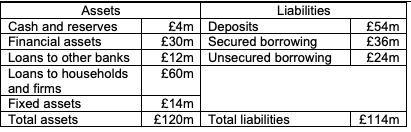
\includegraphics[width=\textwidth]{../QuestionBankImage/OUP-U10-Q23-01.png}

\answer{D}
\begin{tasks}(1)
    \task £34 million of the assets are owned by the bank.
        \details{The bank owns the cash and reserves, the financial assets, and the fixed assets. The loans are owned by the borrowers. Therefore 4 + 30 + 14 = £48 million of the assets are owned by the bank.}
    \task 	The value of the bank’s equity is £120 million.
        \details{The equity is the bank’s net worth, the value of which is 120 - 114 = £6 million.}
    \task The bank’s leverage ratio is 95.
        \details{That would be the leverage ratio normally defined for non-banks (total liabilities/total assets). For banks the leverage ratio is defined as total assets/net worth, which in this case is 120/6 = 20.}
    \task A fall of over 5\% in the asset value would make the bank insolvent.
        \details{The bank’s leverage is 120/6 = 20, meaning that the equity value is only 5\% of the total assets. This means that a fall of over 5\% in the asset value would wipe away its equity, making it insolvent.}
\end{tasks}



\Question
The diagram depicts Marco’s choice of consumptions in periods 1 and 2. He has \$100 worth of grain in period 1 and no income in period 2. Marco has two choices. In scheme 1, he can sell the grain that he does not consume and lend the money at 10\%. In scheme 2, he can invest the grain that he does not consume (e.g. planting as seed) for a return of 50\%. Which of the following statements is correct?
    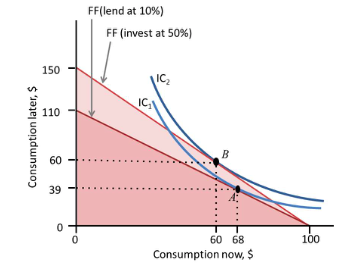
\includegraphics[width=\textwidth]{../QuestionBankImage/OUP-U10-Q12-01.png}
\answer{D}
\begin{tasks}(1)
    \task Marco is less impatient at B than at A.
        \details{The marginal rate of substitution is higher at B than at A. Therefore Marco is more impatient at B than at A.}
    \task Going from scheme 1 to scheme 2, the substitution and income effects have opposite effects on period 2 consumption.
        \details{A higher return means (i) it is more expensive to consume in period 1, and therefore the substitution effect is positive for period 2 consumption, and (ii) higher total income, which implies that the income effect is also positive for period 2 consumption.}
    \task Marco can do better than consumption choice B by investing all of his grain and consuming the output in period 2.
        \details{B is the point of tangency between the scheme 2 feasible frontier and the highest attainable indifference curve. Therefore he would be worse off at any other point on the feasible frontier, including at the ends.}
    \task Marco can do better than consumption choice B by investing all of his grain and borrowing against his period 2 output.
        \details{This shifts the feasible frontier out pivoted at the vertical axis, allowing Marco to attain higher indifference curves than $IC_2$.}
\end{tasks}



\Question
The following diagram depicts Julia’s choice of consumption now and consumption later (next period). She has no income now and an income of \$115 later. The current interest rate is 15\%. Based on this information, which of the following statements is correct?
    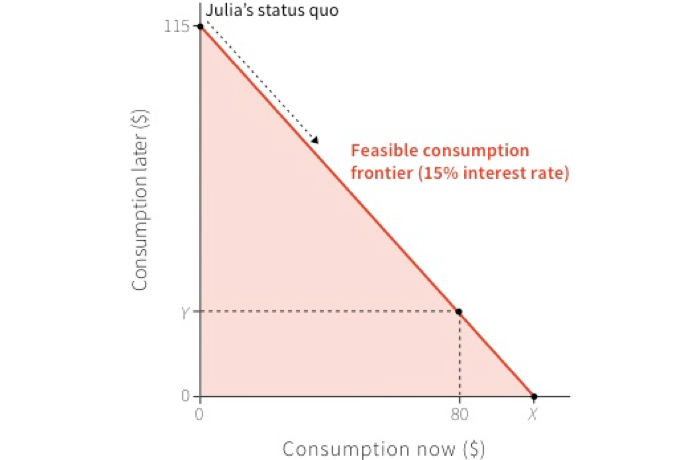
\includegraphics[width=\textwidth]{../QuestionBankImage/TEA-U10-Q2-01.png}
\answer{B}
\begin{tasks}(1)
    \task The maximum that Julia can borrow to spend now is \$91.
        \details{The maximum that Julia can borrow is $\$115/(1 + 0.15) = \$100$. This is the maximum that she can spend now.}
    \task If Julia borrows \$80 to spend now, she will have \$23 to spend later.
        \details{If Julia borrows \$80, she has to pay back $\$80 \times  1.15 = \$92$, so she will have \$115 - \$92 = \$23 to spend later.}
    \task The consumption choice of \$60 now and \$50 later is a feasible option.
        \details{When Julia borrows \$60, she has to pay back $\$60 \times  1.15 = \$69$, so she will have \$115 - \$69 = \$46 to spend later. Therefore the choice (60, 50) is not in her feasible set.}
    \task The feasible set will be smaller when the interest rate is 10\%.
        \details{When the interest rate falls, Julia’s feasible set will become larger: she will be able to borrow a maximum of \$115/(1 + 0.1) = \$104.5 to spend now.}
\end{tasks}



\Question
The diagram depicts Marco’s choice of consumptions now and later (next period). He has \$100 worth of grain now and no income later. Marco has two choices. In scheme 1, he can store the grain that he does not consume now. This results in a loss of 20\% of the grain due to pests and rotting. In scheme 2, he can sell the grain that he does not consume and lend the money at 10\%. Based on this information, which of the following statements is correct?
    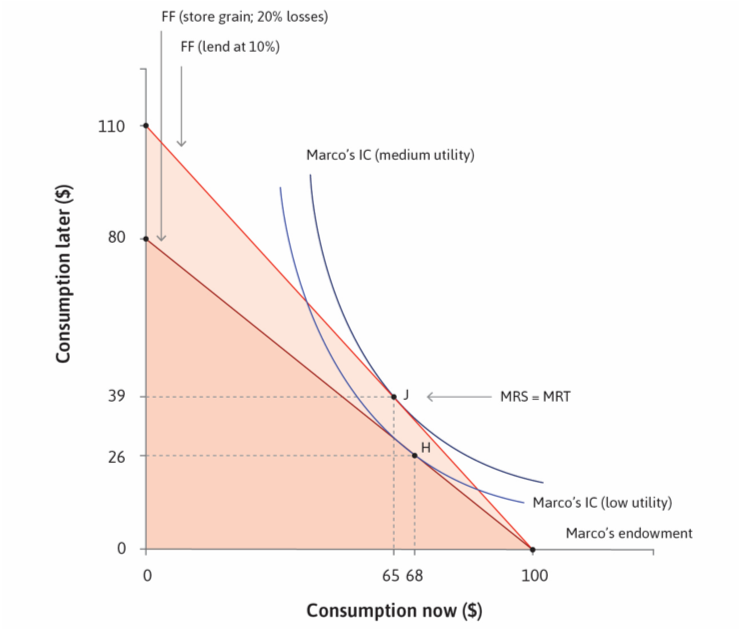
\includegraphics[width=\textwidth]{../QuestionBankImage/TEA-U10-Q5-01.png}
\answer{C}
\begin{tasks}(1)
    \task The substitution effect implies that Marco will consume more now under scheme 2 than under scheme 1.
        \details{The higher MRT in scheme 2 means that Marco will want to consume less now under scheme 2.}
    \task The income effect implies that Marco will consume more later and less now under scheme 2 than under scheme 1.
        \details{The income effect means that Marco will want to consume more in both periods (now and later) under scheme 2.}
    \task Marco will unambiguously consume more later under scheme 2 than in scheme 1.
        \details{The income and substitution effects work in the same direction, so Marco will consume more later under scheme 2.}
    \task Marco will unambiguously consume less now under scheme 2 than in scheme 1.
        \details{This depends on the relative size of the negative substitution effect and the positive income effect. If the latter more than offsets the former then Marco will also consume more now.}
\end{tasks}




\Question
The following diagram depicts Julia’s choice of consumption in periods 1 and 2. She has no income in period 1 and an income of \$115 in period 2. The current interest rate is 15\%. Based on this information, which of the following statements is correct?
    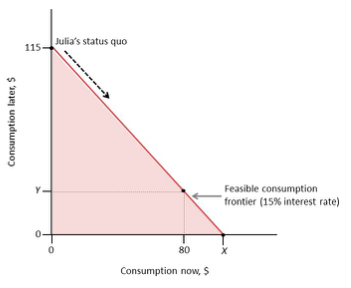
\includegraphics[width=\textwidth]{../QuestionBankImage/UCL-S16-Q6-01.png}
\answer{B}
\begin{tasks}(1)
    \task The maximum that Julia can borrow to spend in period 1 is \$91.
        \details{The maximum Julia can borrow to spend in period 1 is \$100 (= 115/1.15). She borrows \$100, she needs to pay back the principal and \$15 in interest, so in period 2 she will consume \$0 but she will have repaid her debt.}
    \task If Julia borrows \$80 to spend in period 1, she will have \$23 to spend in period 2.
        \details{If she borrows \$80, she is giving up \$80 in period 2, and she will need to pay \$12 in interest. Therefore, in period 2 she will only be able to consume \$115 - (\$80 + \$12) = \$23.}
    \task The consumption choice of \$60 in period 1 and \$50 in period 2 is a feasible option.
        \details{If she borrows \$60, she will need to repay the principal and \$9 in interest. So in period 2 she will only be able to consume at most \$115 - (\$60 + \$9) = \$46. She cannot consume \$50 in period 2.}
\end{tasks}



\Question
Which of the following statements about liquidity and solvency is/are true?
\answer{A}
\begin{tasks}(1)
    \task The relevant items on the balance sheet to assess solvency are total liabilities and total assets.
        \details{Solvency is defined as the value of assets exceeding the value of liabilities, so we need total assets and liabilities in order to assess solvency.}
    \task Allowing banks to borrow from the central bank at a penalty rate of interest can deal with a bank’s solvency but not liquidity problem.
        \details{Borrowing increases a bank's liabilities, so the converse is true: Allowing banks to borrow from the central bank at a penalty rate of interest can deal with a bank’s liquidity but not solvency problem.}
    \task If a bank admits that many of its loans are ‘non-performing’ and unlikely to be repaid, this increases its liabilities.
        \details{Bank loans are on the asset side of its balance sheet, so declaring loans as 'non-performing' increases its assets.}
\end{tasks}

\end{Exercise}

\end{document}
